% Created 2013-04-18 Thu 11:27
\documentclass[11pt]{article}
\usepackage[utf8]{inputenc}
\usepackage[T1]{fontenc}
\usepackage{fixltx2e}
\usepackage{graphicx}
\usepackage{longtable}
\usepackage{float}
\usepackage{wrapfig}
\usepackage{soul}
\usepackage{textcomp}
\usepackage{marvosym}
\usepackage{wasysym}
\usepackage{latexsym}
\usepackage{amssymb}
\usepackage{amstext}
\usepackage{hyperref}
\tolerance=1000
\usepackage[letterpaper, margin=1in]{geometry}
\renewcommand{\maketitle}{}
\author{G. Jay Kerns, PhD}
\date{Spring 2013}
\title{Project/Thesis Template for Graduate Students}
\hypersetup{
  pdfkeywords={},
  pdfsubject={},
  pdfcreator={Emacs 24.3.1 (Org mode 8.0-pre)}}
\begin{document}

\maketitle

%    Copyright (C) 2013 G. Jay Kerns
%
%    Permission is granted to copy, distribute and/or modify this document
%    under the terms of the GNU Free Documentation License, Version 1.3
%    or any later version published by the Free Software Foundation;
%    with no Invariant Sections, no Front-Cover Texts, and no Back-Cover Texts.
%    A copy of the license is contained in the LICENSE file in this 
%    directory.

\newpage
\thispagestyle{empty}
\begin{center}
\textbf{TITLE OF THE PROJECT (all caps)} 

\vspace{0.25in}
by 
\vspace{0.25in}

\textbf{Your Name Here}

\vspace{1in}

Submitted in Partial Fulfillment of the Requirements\\
for the Degree of\\
\vspace{0.1in}
MASTER OF SCIENCE\\
\vspace{0.1in}
in the\\
Department of Mathematics and Statistics\\

\vspace{1in}

\textbf{Graduate Project Committee}\\
\bigskip
Dr.\ G.\ J.\ Kerns (Chair)\\
Department of Mathematics \& Statistics\\
\bigskip

Dr.\ Second Member\\
Department of Mathematics \& Statistics\\
\bigskip

Dr.\ Third Member \\
Department of Maybe Another Department\\

\vfill
YOUNGSTOWN STATE UNIVERSITY\\
May, 2013 
\end{center}

\newpage
\pagenumbering{roman}
\setcounter{page}{2}
\begin{center}
\textbf{ABSTRACT} 
\end{center} \vspace{0.25in}

Type the text of your Abstract here.  It should be a one page, 
concise description of your project. It should be self-contained, 
and a person should be able to read this one page and get a very 
good idea about the subject and main results of your project. 
This section should not contain cross-references to any other 
paper or book. 

\newpage
\begin{center}
\textbf{ACKNOWLEDGEMENTS} 
\end{center} \vspace{0.25in}

This page is optional. If desired, you may acknowledge those 
individuals that played a significant role in your successful 
completion of the project. If you are going to have this page, 
then you should make sure to include the YSU Department of 
Mathematics and Statistics, and of course, your project advisor 
and committee members.

\newpage
\tableofcontents

\newpage
\section[Introduction]{Introduction}
\label{sec-1}
\pagenumbering{arabic}

The goal in this section is to introduce the reader to the subject of
your project. This is the place for relevant background information
that a person should know in order to put your project in
context. Discuss any prior history or work that has been done on this
topic. Define any essential terms or concepts from other fields that
are used throughout the paper.

Most of your literature review will be mentioned here. Every time that
you reference a paper, be sure to add a citation, for instance, Efron
\cite{Efron1972}. In order to cite properly, your References section
needs to be current, consistent, and complete; see \cite{Cons} and
\cite{NoCopy} at the end of this document.

\newpage

\section[Overview]{Overview}
\label{sec-2}

This section gives a bird's eye view of your project, as a whole.  You
have introduced the reader to all of the necessary background for your
project in Section \ref{sec-1}, so now (s)he is ready to learn,
in broad terms, what you did in your project and how all of the pieces
fit together.

It is not appropriate to include many minute details in this
section. It is fine to include graphs, but they should only be used in
the context of communicating the main ideas of your project. Lengthy
tables and lists of variables or p -values are not appropriate; those
should be saved for Section \ref{sec-4}, Analysis.

It is appropriate to mention the main research questions that you are
investigating with this project, but save the answers and details for
Sections \ref{sec-4}, \ref{sec-5}, and \ref{sec-6}.

\subsection[Project Timeline]{Project Timeline}
\label{sec-2-1}

This is set apart so that you can see what a subsection looks like
inside of a section. The list below is typeset with a Description
environment. It describes a basic time-line for you while completing
your project.

\begin{description}
\item[Beginning of semester or earlier:] Schedule meetings with
potential advisers to see if they are available to do a project
with you. Bring to the meeting ideas of topics/subjects that you
would like to study. Prepare a list of the MATH/STAT courses you
have had at YSU. Leave the meeting with two or three
possibilities of projects for you to investigate. Be prepared to
go to the library or Internet to find data related to the
topic(s) discussed.
\item[Second meeting:] Bring example data sets to the meeting, for
discussion and selection. Choose a project adviser and project
topic. Ask your adviser about potential professors to serve on
your project committee, and then approach the candidates to ask
them (politely) if they are willing/able to serve on the
committee. Keep searching until you find two professors who
accept.

\item[Third meeting:] Bring your class schedule, and set up regular
weekly meeting times with your adviser. Notify
your adviser of the additional committee
members. Schedule a tentative date for the
computer lab for your project presentation and
defense.  This will be Presentation Day, and
should be scheduled for at least one week prior to
the beginning of Final Exams. After the meeting,
speak with the other committee members to revise
or confirm the presentation day.
\item[Two weeks prior:] PROJECT REPORT DUE DATE. Give a final, printed
copy of the document to each of your committee members. Begin
preparation for your presentation by making PowerPoint slides of
your project work. Organize your presentation in the same way
that this document is organized.

\item[One week prior:] Meet with your adviser to discuss your
presentation slides. Rehearse your presentation by yourself, with
a clock to time the length of the delivery. Send your adviser an
email containing the title of the presentation and an abstract,
for announcement to the department faculty.

\item[One day prior:] Prepare a notice containing the time, place, and
title of your presentation. Make copies and post
them in the Math office and on the office suite
doors.

\item[Presentation Day:] Good luck! Do a great job!

\item[Immediately afterward:] Make sure that the projector and other
equipment are secured and returned to their original
location(s). Remove the notices from the doors. Meet with your
adviser to discuss revisions to the document which have been
suggested by the committee.

\item[Three days afterward:] Give your adviser a printed copy of the
final, revised draft of the document for the adviser to review.

\item[After approval:] Give a three-ring bound final copy to Sandi, the
Mathematics \& Statistics Secretary. You may also wish to give
your adviser a bound copy.

\item[TO GRADUATE:] Very important! If you did not finish your project
in one semester, then you recieved a grade of "In
Progress" (PR) in the semester in which you
registered for your project.  In order to graduate,
this grade must be changed using special
paperwork. You need to go to Sandi, the Mathematics
\& Statistics secretary, and request a “Change of
Grade” form. She will give you instructions for
filling out the form. Submit the completed form to
your adviser, who will fill in the remaining
details. If this form is not completed, you will not
graduate.  It is your responsibility to make sure
that all of the procedures are followed in a timely
manner.
\end{description}

\newpage

\section[Methodology]{Methodology}
\label{sec-3}

The goal in this section is to lay the theoretical foundation of the
later sections. You will be doing a lot of computations in Section
\ref{sec-4}, and you will want to include here a discussion of each
of the main procedures that you will be using.  For example, if you
are doing a project with multiple regression analysis, then you should
discuss the theory of the regression model in this section, together
with the model's assumptions. If your project is a cluster analysis of
some data, then you should detail the algorithms/methods that were
used and their properties and weaknesses.

If you use certain statistics to perform a hypothesis test or assess
the accuracy of a particular procedure, then they should be quoted
here (with their respective formulas). Again, discuss their strengths
and weaknesses, and make it clear why you chose them. If there are any
special probability distributions that you are using, then you should
include them here, with formulas, and describe their connection to the
topic you are studying.

\subsection[Mathematical Typesetting]{Mathematical Typesetting}
\label{sec-3-1}

Given that you are a student in the Department of Mathematics \&
Statistics, the probability is high that you will want to include
mathematical notation and formulas in your report, and they are
entered using a special \LaTeX{} math mode. There are three primary ways
to do this.

The first way is called an "inline formula", which means that the
formula is included in the text with everything else. An example would
be \(f(x)\) or \( \int\sin x\ \mathrm{d}x \). This way is handy when
mentioning variables or short expressions.

The second way is called a "displayed formula", which is separated
from the rest of the text in its own displayed paragraph. An example
would be
\[
f(x)=\frac{1}{\sqrt{2\pi}}\mathrm{e^{-x^{2}/2},\quad-\infty<x<\infty},
\]
which is useful for longer formulas or equations. 

The last way is a "numbered formula", which displays the formula
labeled with a number, for instance,

\begin{equation}
\mathrm{e}^{i\pi}-1=0.
\end{equation}

There can be many of these in a the document, and the equation numbers
will be generated automatically by LyX.

Please note that there are many, many, many things that can be done
with \LaTeX{} and mathematics. Do a Google search for "latex math
examples" for a taste.

In particular, all variables, functions, and expressions in the
document should be written in math mode. It is not acceptable to write
X or Y when discussing variables in your report\ldots{} they should instead
be \(X\) and \(Y\) so that the reader can easily distinguish between
mathematics and text.
\subsection[Copying Material from the Internet (or elsewhere)]{Copying Material from the Internet (or elsewhere)}
\label{sec-3-2}

This document is yours, and the reader will assume that all of the
words in it were written by you unless something special indicates
otherwise. Take, for instance, this quote from Fox \cite{Fox2002}
which discusses the bootstrapping technique:

\begin{quote}
Bootstrapping is a general approach to statistical inference based on
building a sampling distribution for a statistic by resampling from
the data at hand. The term "bootstrapping," due to Efron
\cite{Efron1972}, is an allusion to the expression "pulling oneself up
by one’s bootstraps" -- in this case, using the sample data as a
population from which repeated samples are drawn. At first blush, the
approach seems circular, but has been shown to be sound.
\end{quote}

Notice that the above quotation environment makes it immediately
obvious to the reader that the words in the separate paragraph were
written by John Fox, and not by me. Any passages that are copy/pasted
into this document must be set apart in a quotation environment, just
like the one above. If there is even a sentence in the document that
you have copied from the Internet (or elsewhere, such as a book or
journal) which is not set apart and referenced, then you have
committed plagiarism, a very serious offense at this level of your
academic career. Be careful about quoting external material.

Rather than copying someone else's writing into your project, it is
better to read the material and write another version in your own
words. Try to paraphrase the material into a shorter version that
makes sense to you, or alternatively go in the other direction by
adding explanations that the original author skipped. The goal is to
make the passage your own.

There are exceptions: mathematical definitions, being one. These are
quoted everywhere and are contained in many texts and references. It
is not necessary to quote/reference a definition, unless the specific
definition warrants otherwise. Ask your adviser concerning any cases
about which you are unsure.

\newpage

\section[Analysis]{Analysis}
\label{sec-4}

This section is the "meat" of the project. It is here that you present
your computations, tables, scatterplots, diagnostic graphs, and
\emph{p}-values. You will spend the majority of the time working on the
results to put into this section. It is appropriate to include

\begin{enumerate}
\item The source of the data set, including its size, the number of
variables, the types of the variables, and the format in which you
received/collected the data.
\item Summary descriptive statistics of the data. For quantitative
variables, address the center, spread, shape, and unusual features
of the data distribution. Graphical displays include boxplots,
histograms, scatterplots, etc. Identify outliers. For categorical
data, summary frequency distributions and bar charts or dotplots
are appropriate.
\item A discussion of the model fitting, or the other major purpose of
your project. List all assumptions being made.
\item Diagnostic checks of your fitted model. Does the model fit well?
Are the assumptions satisfied? Employ remedial measures if
necessary, and repeat.
\item A practical application of your fitted model or procedure,
something useful, the main goal of your project. Assess the
adequacy of your model with a measure of model performance.
\end{enumerate}

Do not spare any details for the reader in this section. If (s)he has
a question about a statement made elsewhere in the paper, (s)he will
come here to sift through the results for an answer.  If the answer is
not buried here, then the validity of your paper will be compromised.

\begin{figure}[ht]
\centering
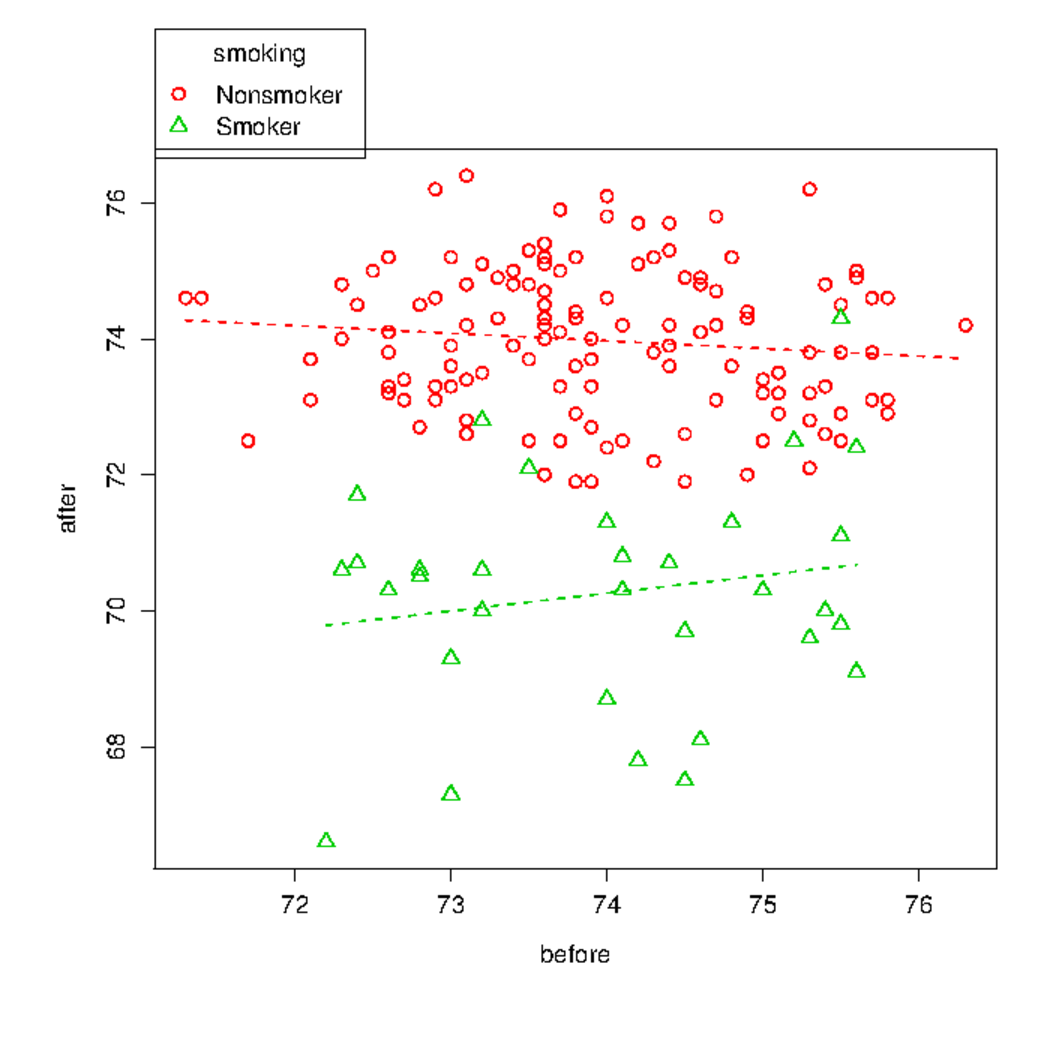
\includegraphics[width=0.90\textwidth]{examplefig.pdf}
\caption[A scatterplot]{\label{fig-scatterplot}\small Scatterplot of \texttt{after} vs. \texttt{before} by smoking status.}
\end{figure}
\subsection[Graphs and Displays]{Graphs and Displays}
\label{sec-4-1}

The Analysis section will likely have many graphs and displays. 
Here are some general considerations to keep in mind:

\begin{itemize}
\item Every graph should be labeled "Figure", with a respective figure
number, and an accompanying descriptive title. If you are using LyX
to typeset your document, then every figure should be enclosed in a
"Figure float", in which case these labels will be generated
automatically.
\item Every graph or display should be referenced in the main body of the
text, and should have at least a paragraph describing what the
figure is and the figure's salient features. If you can't come up
with even a paragraph of important things to say about the picture,
then the picture is not worth including in the project report.
\item Every graph should be a maximum of 1/2 page in size, except in very
rare circumstances\footnote{Some graphs are simply too big to fit in 1/2 page and still be
legible without a magnifying glass. As of 2013, I have only
encountered two (2) graphs in graduate projects which I have supervised
that merited their own page.}. In addition, try to avoid putting two (2) graphs
on one (1) page; rather, put the graphs on two separate pages and
include a description underneath of each one. See the previous
bullet.
\end{itemize}

An example of a properly labeled graph is included as Figure \ref{fig-scatterplot} (but the paragraph is missing).
\subsection[Tables]{Tables}
\label{sec-4-2}

DO NOT COPY/PASTE TABLES FROM SPSS\(\circledR\). The tables returned
by most software packages are overly complicated and are full of
irrelevant information. If you have a generated table that you would
like to include, take a close look at it and identify the essential
information that you need to convey your point. Next, retype (or
export) that information in a table, properly referenced, in the main
body of the document. An example of a good table is included below as
Table \ref{tab-gender}.  Note that it has been enclosed in a table float,
which is analogous to a figure float.

\begin{table}[htb]
\caption{\label{tab-gender}\small Tabular results of \emph{Ethnicity} versus \emph{Gender}.}
\centering
\begin{tabular}{llrrr}
 &  &  & \emph{Gender} & \\
 &  & Female & Male & Total\\
\hline
\emph{Ethnicity} & Caucasian & 15 & 4 & 19\\
 & African American & 31 & 7 & 38\\
 & Asian/Pacific Islander & 8 & 1 & 9\\
 & Hispanic & 16 & 1 & 17\\
 & Other & 4 & 3 & 7\\
\hline
Total &  & 74 & 16 & 90\\
\end{tabular}
\end{table}

Note that there has been a deliberate attempt to use dividing lines
sparingly in the table. Try not to put too many lines; they end up
making your table more difficult to read.

The previous remarks made about figures also apply to tables.
\begin{itemize}
\item Every table should be labeled and numbered, with a descriptive
title.
\item Every table should be referenced in the main body of the text with a
corresponding descriptive paragraph, at least.
\item Avoid especially large tables, if possible. Some tables may be
safely relocated to the Appendix.
\end{itemize}

\newpage

\section[Discussion]{Discussion}
\label{sec-5}

In Section \ref{sec-4} you included many tables, graphs, displays,
and calculations. In the Discussion section, the goal is to make sense
of the results presented in the Analysis. Take a step back from the
details and try to address: “What are the data telling us?” Try to put
the results in context, and discuss the implications of the results
that you found.

It is appropriate in this section to admit problems that you faced
with the data, and limitations to your study. If the data do not
support your original hypothesis, then say so. It is better to admit
weaknesses of your study up front, rather than try to conceal them and
hope that no one notices, or even worse, to ignore the weaknesses
entirely. Spending time thinking critically and reflectively about the
results will strengthen the project overall.

\newpage

\section[Conclusion]{Conclusion}
\label{sec-6}

This is it! The Conclusion section is the end of the road, the
location to which all other sections are pointed. Think of this
section as an expanded and less concise version of your ABSTRACT.  The
reader should be able to read the Conclusion and have a complete
picture of the main questions which led you to this project, and the
answers that you found.

\newpage
\appendix
\section[Supporting Documentation]{Supporting Documentation}
\label{sec-7}

Every project is unique. However, in nearly every project there is
additional information which supplements the discussion in the main
narrative but whose inclusion would clutter the paper
needlessly. Place this extra material here. It could include
additional graphs, lengthy tables, background mathematical theory,
etc.
\section[Complete R and SAS\(\circledR\) Scripts]{Complete R and SAS\(\circledR\) Scripts}
\label{sec-8}

You should collect all of the computer code that you used at any point
in your project and post it in this section. There will certainly need
to be some cleanup of the code to make it legible to the reader, but
do not delete too much. The reader should be able to take the code
from your project and repeat the analysis, verbatim. It is a good idea
to make a final test-run of the code in this section to make sure that
there aren't any crucial steps missing.

Remember: all computer code/listings should be in a monowidth font
(such as Courier) and not in a proportional font (such as Times
Roman). For instance, you should write \texttt{summary()} instead of
summary().

\bigskip

\textbf{About this document:} (the below was typeset in the \texttt{verse}
environment)

\begin{verse}
Last modified: April 17, 2013 \\
Author: G. Jay Kerns, Ph.D. \\
Typeset with: Org mode \texttt{8.0pre} in GNU Emacs \texttt{24.3.5.1} \\
Electronic versions in (\texttt{.org}, \texttt{.lyx,=, .tex}, \texttt{.pdf}) \\
formats can be downloaded from \href{https://github.com/gjkerns/gradproject}{GitHub} \\
\end{verse}

\phantomsection
\addcontentsline{toc}{section}{References}
\bibliographystyle{plainurl}
\bibliography{gradproject}
% Emacs 24.3.1 (Org mode 8.0-pre)
\end{document}